\documentclass[a4paper,french]{paper}
\usepackage{../../../../../_assets/latex/5N_OPTO_ELEC}

%Informations about this document 
%------------------------------------------
\def\module{Opto-Electronique - S5}
\def\moduleAbrege{5N-027-SCI / OptoElec}
\def\annee{2024-2025}

\def\titre{Séance 3 / Filtrage d'un signal électrique}
\author{Julien VILLEMEJANE}

\subtitle{Séance 3}
\institution{LEnsE / Institut d'Optique Graduate School}

\title{\titre}
\begin{document} 
%Beginning First Page. 
%------------------------------------------
\enteteThematiqueObligatoire{}

\textit{Pour ce TD, on pourra s'appuyer sur les fiches résumées} : \href{https://lense.institutoptique.fr/ressources/Annee1/Electronique/fiches/2020_FR_RegimeHarmonique.pdf}{Régime Harmonique}, \href{https://lense.institutoptique.fr/ressources/Annee1/Electronique/fiches/2021_FR_ALI.pdf}{Ampli Linéaire Intégré} et \href{https://lense.institutoptique.fr/ressources/Annee1/Electronique/fiches/2020_FR_FiltreOrdre1.pdf}{Filtre d'ordre 1}

%Beginning Content. 
%------------------------------------------

%%%%%%%%%%%%%%%%%%%
%%%%%%%%%%%%%%%%%%%
\encadreTDExo{3.1 - Charge et décharge d'un condensateur}{

Soit le circuit suivant :

\begin{center}
\begin{circuitikz}
	\draw (0,0) to [R=$R$, o-*] (3,0)
		to[C=$C$, -*] (3,-3)
		to[short, -*](1,-3)
		node[ground](GND){}
		to[short, -o](0,-3);
	\draw (3,0) to[short, -o](4,0);
	\draw (3,-3) to[short, -o](4,-3);
	% fleche
	\draw (0,-2.7) edge[->] (0,-0.3);
	\node (Ein) at (-0.5,-1.5){$V_E$};
	% fleche
	\draw (4,-0.3) edge[<-, green!40!black] (4,-2.7); 
	\node[text=green!40!black] (US) at (4.5,-1.5){$V_S$};
\end{circuitikz}
\end{center}

\begin{enumerate}
	\item Donnez le lien entre $V_E(t)$ et $V_S(t)$.
	\item Donnez l'expression de $V_S(t)$ pour $t > 0$ pour $V_E(t) = E$ (constante). On supposera le condensateur totalement déchargé à $t = 0$ (c'est à dire si $V_S(0) = 0$) et tracez $V_S(t)$.
	\item Donnez le protocole de mesure de la \textbf{réponse indicielle} de ce circuit. 
\end{enumerate}
}

%%%%%%%%%%%%%%%%%%%
%%%%%%%%%%%%%%%%%%%
\encadreTDExo{3.2 - Filtre analogique d'ordre 1}{

On reprend le schéma de l'exercice précédent (exercice 3.1), mais cette fois-ci, nous nous plaçons dans un régime harmonique. Ce circuit est alors alimenté par une source de tension sinusoïdale de pulsation $\omega_0$. On prendra $R = 1\operatorname{M\Omega}$ et $C = 100\operatorname{nF}$.

\begin{enumerate}
	\item Déterminez la \textbf{fonction de transfert} $T( j\omega ) = V_s / V_e$ en fonction de la pulsation et des éléments du montage.
		
	\item Déduisez la \textbf{pulsation de coupure} $\omega_0$ de $T( j\omega )$ et le \textbf{gain dans la bande-passante} en fonction des éléments du montage.

	\item Tracez le \textbf{diagramme de Bode} du gain et de la phase en fonction de la pulsation.

	\medskip
	
	On réalise la réponse en fréquence de ce système expérimentalement à l'aide d'un générateur de fonction ($R_s = 50\operatorname{\Omega}$) et d'un oscilloscope numérique ($R_e = 1\operatorname{M\Omega}$).
	
	Après analyse, nous obtenons une fréquence caractéristique $\omega_c = 20\operatorname{rd/s}$ et une amplification dans la bande passante de 0.5.
	
	\item Proposez une explication à ces résultats.
	
	\medskip
	
	\item On met deux étages de ce type en \textbf{cascade}. Quelle est la fonction de transfert alors obtenue ?

\end{enumerate}
}

%%%%%%%%%%%%%%%%%%%
%%%%%%%%%%%%%%%%%%%
\encadreTDExo{3.3 - Filtre universel}{

%%%%%%%%%%%%%%%%%%%
\textbf{Bloc intégrateur}

On se propose d'étudier la réponse du système suivant :

\begin{center}
	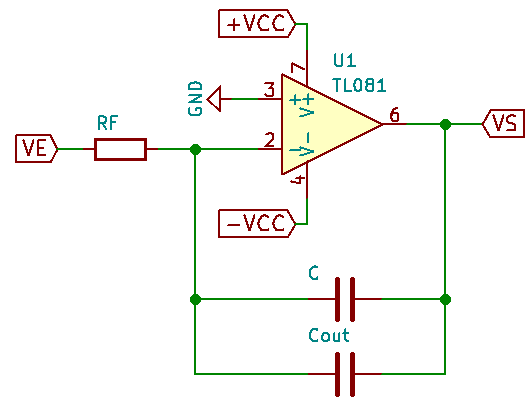
\includegraphics[width=8cm]{images/universel_integrateur.png}
\end{center}

Donner la relation entre $V_S$ et $V_E$.

\centerline {\rule{.5\linewidth}{.25pt}} % Horizontal line
%%%%%%%%%%%%%%%%%%%
\textbf{Bloc additionneur}

On s'intéresse à présent au bloc suivant :

\begin{center}
	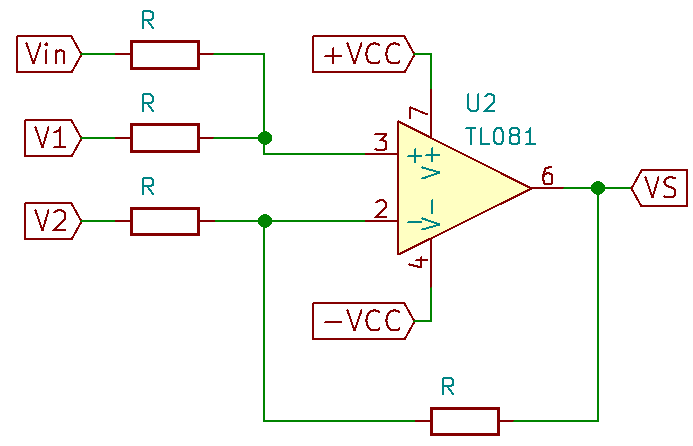
\includegraphics[width=8cm]{images/universel_sommateur.png}
\end{center}

Donner la relation entre $V_S$, $V_1$, $V_2$ et $V_{in}$.


\centerline {\rule{.5\linewidth}{.25pt}} % Horizontal line
%%%%%%%%%%%%%%%%%%%
\textbf{Structure universelle}

Soit la structure suivante, basée sur les montages vus précédemment :

\begin{center}
	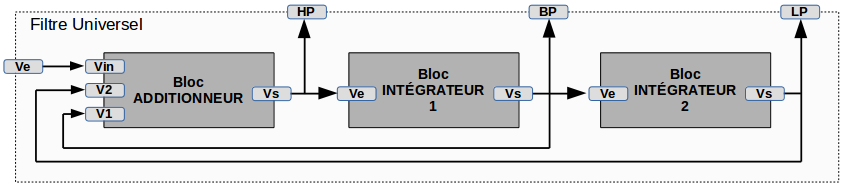
\includegraphics[width=12cm]{images/universel_structure.png}
\end{center}

\begin{enumerate}
	\item Calculer $V_{HP}$ en fonction de $V_{in}$ et des divers composants.	
	\item Calculer $V_{BP}$ et $V_{LP}$.	
	\item Que peuvent signifier les noms donnés aux signaux de sortie ?
\end{enumerate}
}

%%%%%%%%%%%%%%%%%%%
\encadreTDExo{3.3 - Filtre universel (suite)}{
%%%%%%%%%%%%%%%%%%%
\textbf{Etude du composant UAF42}

On souhaite s'intéresser au composant UAF42, dont quelques pages de documentation technique sont données en annexe.

\begin{enumerate}
	\item Retrouve-t-on la structure étudiée précédemment dans le schéma de la page 1 de la documentation technique ?
	\item Le câblage de la figure 1 de la page 6 de la documentation technique est-il conforme à la structure universelle proposée précédemment ?
	\item Retrouve-t-on la fonction de transfert calculée précédemment ?
	\item Que doivent valoir $R_{F1}$ et $R_{F2}$ pour obtenir une pulsation de coupure de $30~10^3\operatorname{rd/s}$ ?
\end{enumerate}
}

%%%%%%%%%%%%%%%%%%%
%%%%%%%%%%%%%%%%%%%
\encadreTDExo{3.B1 - Impact des ALI}{
On se propose d'étudier le montage suivant : 

\begin{center}
\begin{circuitikz}
	\draw (0,0) node[above]{} ++(1,0) node[ground](GND){}
	node[op amp, noinv input up, anchor=+, fill=blue!10!white](OA){\texttt{AOP1}}
	(OA.-) to[short,-, i<_=$i^-$] ++(0,-1) coordinate(FB) 
	to[R=$R_1$, i=$I_1$] ++(-2,0) to[C=$C$, -o] ++(-2,0) 
	(FB) to[R=$R_2$, *-] (FB -| OA.out) to[short,-, i<_=$I_2$] (OA.out)
	to [short, *-o] ++(1,0) node[above]{};
	\draw (-3,-2.3) edge[<-,color={green!40!black}] (-3, -4);
	\draw (-3,-4.3) to[open,-o] ++(0,0) node[ground](GND){};
	\node[text={green!40!black}] (Ve) at (-3.5,-3.3){$V_E$}; 
	\draw (4.3,-1) edge[<-,color={red}] (4.3, -4);
	\draw (4.3,-4.3) to[open,-o] ++(0,0) node[ground](GND){};
	\node[text={red}] (Vs) at (4.8,-2.7){$V_S$}; 
\end{circuitikz}
\end{center}

\begin{enumerate}
	\item Donnez la fonction de transfert de ce montage dans le cas des hypothèses classiques sur les amplificateurs intégrés (régime linéaire en particulier : $V^+ = V^-$).

	\item Donnez la fonction de transfert de ce même montage en faisant l'hypothèse que la relation qui régit l'amplificateur linéaire est la suivante : $V_S = A_0 \cdot (V^+ - V^-)$. 

	\item Donnez la fonction de transfert de ce même montage en faisant l'hypothèse que la relation qui régit l'amplificateur linéaire est la suivante : $V_S = A(j\omega) \cdot (V^+ - V^-)$. 
	
	On prendra $$A(j\omega) = \frac{A_0}{1 + j \omega / \omega_0}$$
	
	\item Expliquez alors la différence de comportement obtenu entre les 3 modélisations.
\end{enumerate}
}



%%%%%%%%%%%%%%%%%%%
%%%%%%%%%%%%%%%%%%%
\encadreTDExo{3.B2 - Filtre à capacité commutée}{

Nous allons nous intéresser à présent à des filtres dont la fréquence de coupure est pilotable par un signal extérieur.

%%%%%%%%%%%%%%%%%%%%%%%%%%%%%%%%%%%
\textbf{Capacité commutée}

On donne dans un premier temps la structure suivante, dont l'interrupteur $K$ est piloté par le signal de commande ci-dessous :

\begin{center}
	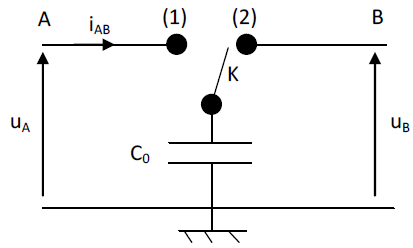
\includegraphics{images/capa_comm.png} 
	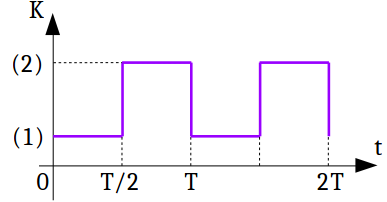
\includegraphics{images/capa_comm_signal.png}
\end{center}


\medskip

\begin{enumerate}
	\item Calculer la charge stockée dans $C_0$ entre les instants 0 et $T/2$, puis entre les instants $T/2$ et $T$.
	\item Quelle quantité de charges passe de A vers B entre les instants 0 et T ?
	\item Calculer alors le courant moyen circulant du point A au point B pendant une période T. 
	\item Donner l'expression de la résistance équivalente $R_{AB}$ vue entre les bornes A et B de cette cellule.
\end{enumerate}


\centerline {\rule{.5\linewidth}{.25pt}} % Horizontal line
%%%%%%%%%%%%%%%%%%%%%%%%%%%%%%%%%%%%%%%%%%%%%%%%%%%%%%%%%%%%%%%%%%
\textbf{Intégrateur à capacité commutée}

On réalise un intégrateur à partir du circuit de la figure 2.

\begin{enumerate}
	\item Donner la fonction de transfert du circuit $T(j\omega) = u_2/u_1$ en fonction de $R_{AB}$ et de $C$.


\begin{center}
	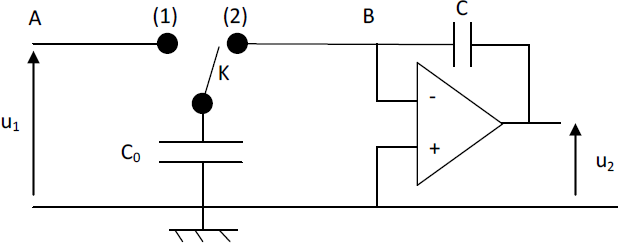
\includegraphics{images/capa_comm_integrateur.png}
\end{center}

	\item Que devient alors la fonction de transfert $T(j\omega{}) = u_2/u_1$ en fonction des éléments du système ($C_0$ et $C$) ?

	\item Quel est l'intérêt d'un tel circuit ?
\end{enumerate}
}

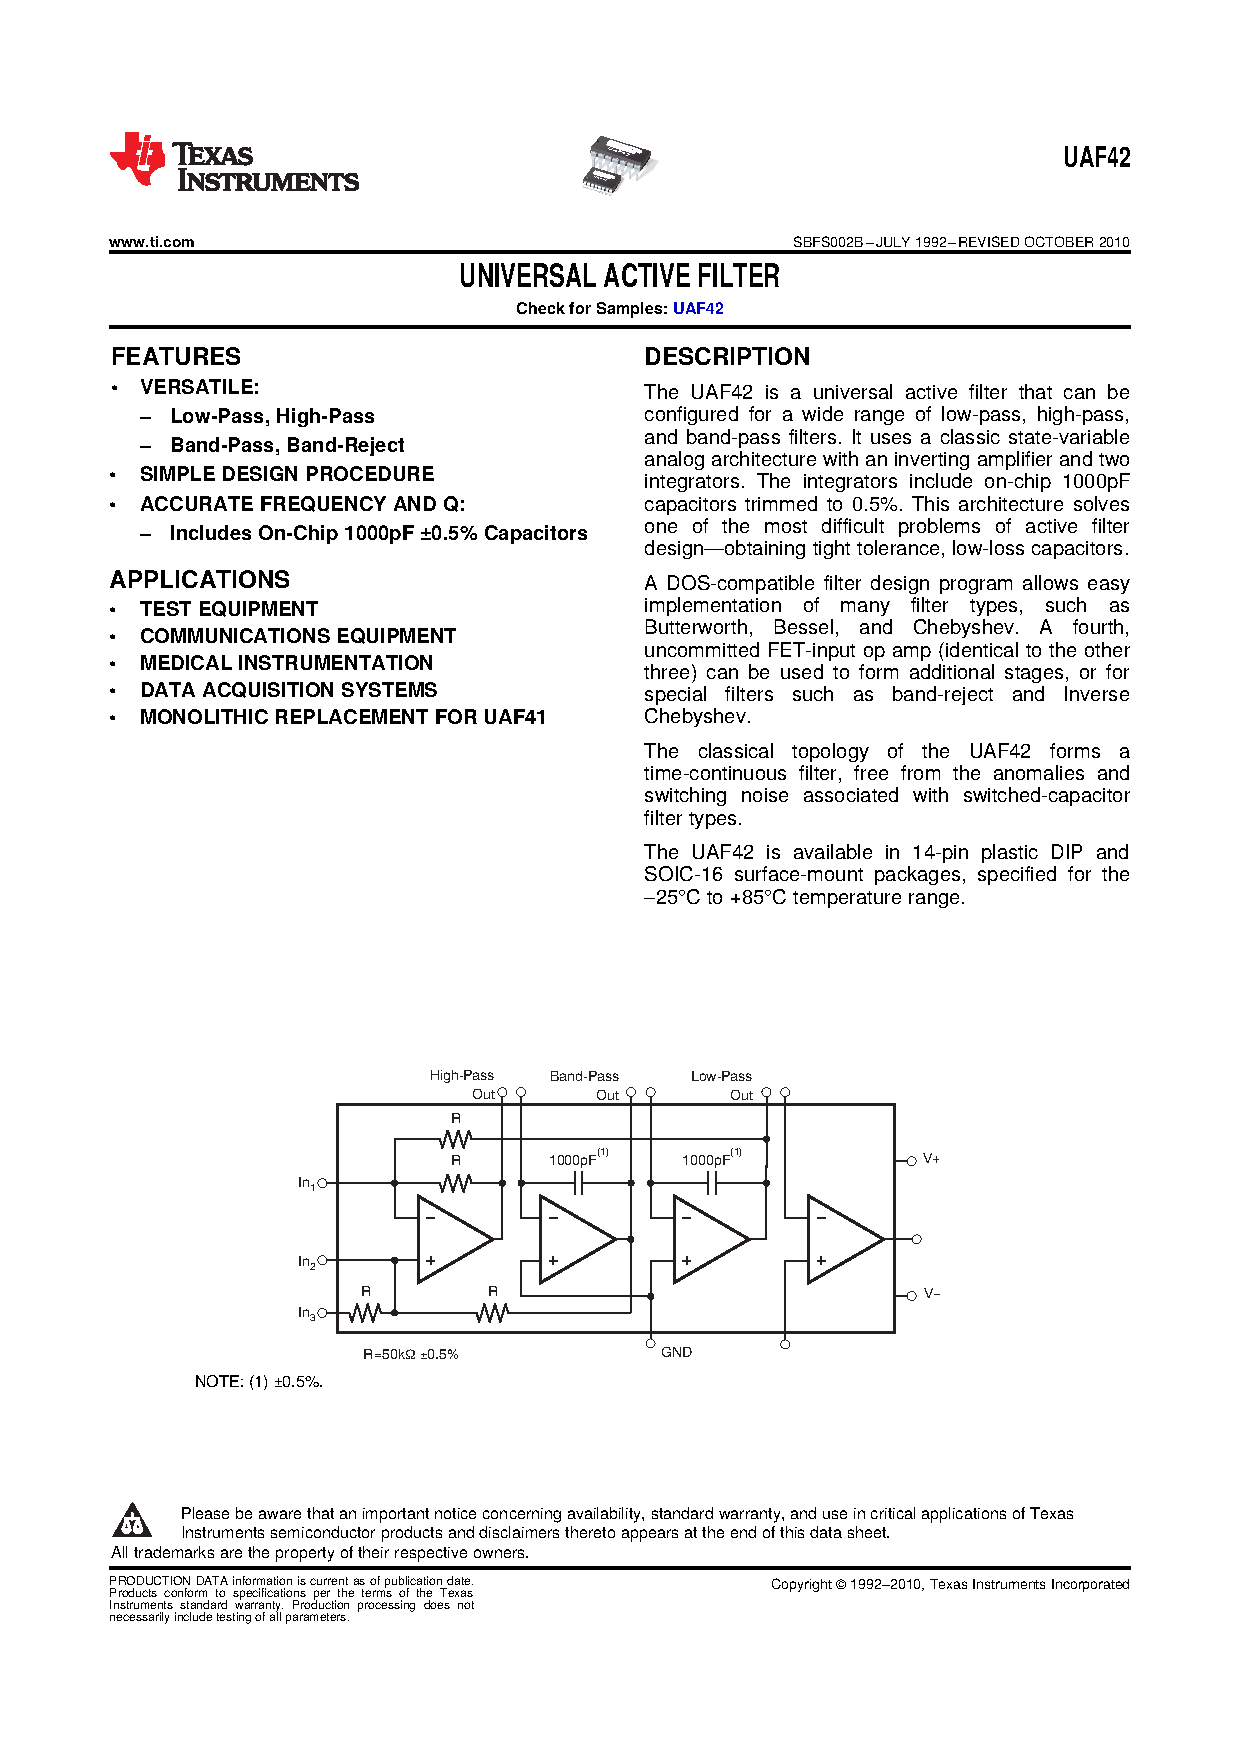
\includepdf[pages=-]{docs/uaf42.pdf}

\end {document}